\documentclass[]{article}
\usepackage[total={7in,9in}]{geometry}
\usepackage[utf8]{inputenc}
\usepackage{graphicx}
\usepackage{hyperref}



\title{PredictingWaterQuality}
\author{Oguzhan SAHIN-Ozgur DOGAN-Dilara SAHAN}
\date{January 2021}

\begin{document}

\maketitle

\section{Abstract}
Humanity have some fundamental needs for existing and the most important of these is water. However, some people continue to pollute lakes, seas and oceans. Water pollution is mostly a result of oil spills and industrial wastes. On the other hand, studies are carried out in many areas to prevent water pollution. When we heard about the presence of algae that clean water and increase the water quality , we decided to focus on this issue. In this project, we aimed to create a model that predicts which waters needed this algae.
\section{Method}
\subsection{Data Collection}
After identifying our problem, first we focused on data collection, which is the most important part of our ML pipeline. For this, we first looked for data that we can work on that shows water quality and decided to use the data europa water pollution data set. Since most features will not be effective for the model, we dropped most of them and decided to add new features. Accordingly, we decided to use WorldBank, SEDAC, Foursquare and OSM (OpenStreetMap) data. The data we add is as follows.

\begin{figure}[h]
    \centering
    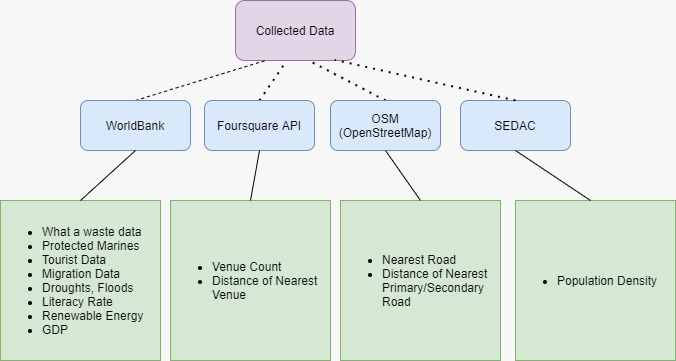
\includegraphics[width=15cm]{CollectedData.png}
\end{figure}
\subsection{Data Preparation}
Since the data we collect is generally country-based, we first obtained country information from the coordinate information on our main water pollution dataset. We have joined data according to this country information. Apart from this ready-to-use data, we decided to use the FourSquare API to detect venues close to the given coordinates, and the OSM API to detect nearby main roads, secondary roads and motor paths. But did not use the OSMnx package due to the lack of computational power.
\subsection{Data Preprocessing}
We combined the different data we collected in a table and made our last studies / tests on this dataset. First of all, we applied normalization because we wanted to get rid of the effect of outliers in the data set. Some outlier values were removed manually from the data set. Then, because categorical data poses a problem, we converted the categorical data into numeric classes with the Label encoder, and we dropped the nan values in the data because they were almost non-existent.
\subsection{Data Exploration}
After finalizing the data, we analyzed and visualized the data in order to understand the connections and patterns within the data. Here is some analysis:
\subsubsection{Analysis Data}
If we need to analyze the data quickly, the final version of the data contains 20k tuples and 29 features. If we need to look at the data types of these 29 attributes, we have 8 categorical and 21 numeric data types. Among these 29 features, the column we will use as the target is the "resultMeanValue" column that contains a continuous data.
\begin{figure}[h]
    \centering
    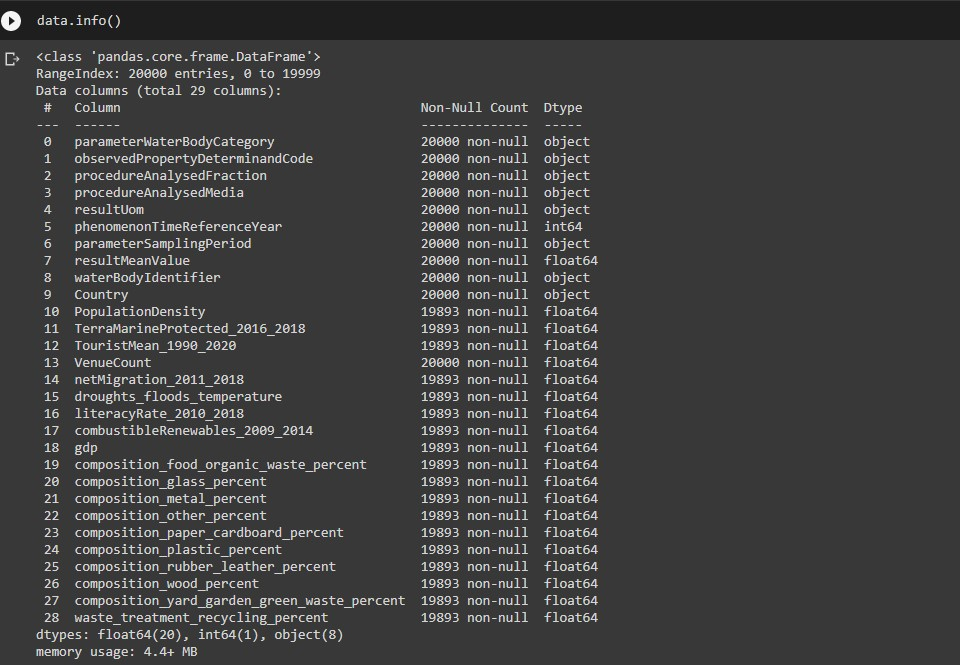
\includegraphics[width=16cm]{dataInfo.jpg}
\end{figure}
As stated in the data preprocessing section, we decided to delete the rows with these values since there are almost no NaN values in the data set. If there were more we could have preferred to fill in these NaN values, but their small number pushed us to this method.
\subsubsection{Visualization Data}
We made visualizations using a Seaborn, Matplotlib and Folium libraries to better understand the data. Our first visualization was on the distribution of water samples taken across countries. Since the raw version of the data set contains more than 2 million data, we had to make certain clippings. Most of the last remaining data are in the regions of France, England and Spain.You can access all the visualizations we have made on the EDA notebook in the github repository.
\begin{figure}[h]
    \centering
    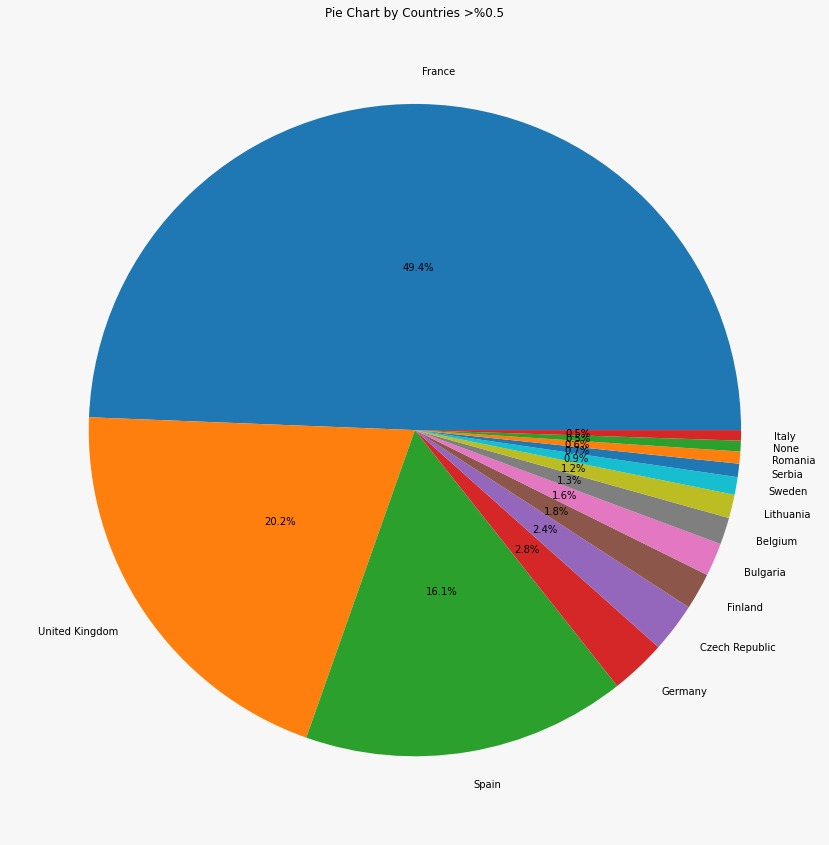
\includegraphics[width=11.5cm]{dataByCountries.png}
\end{figure}
 In addition, we visualized these data on a map according to their coordinates with the help of the Folium library to learn how the samples are distributed on the map.
\begin{figure}[h]
    \centering
    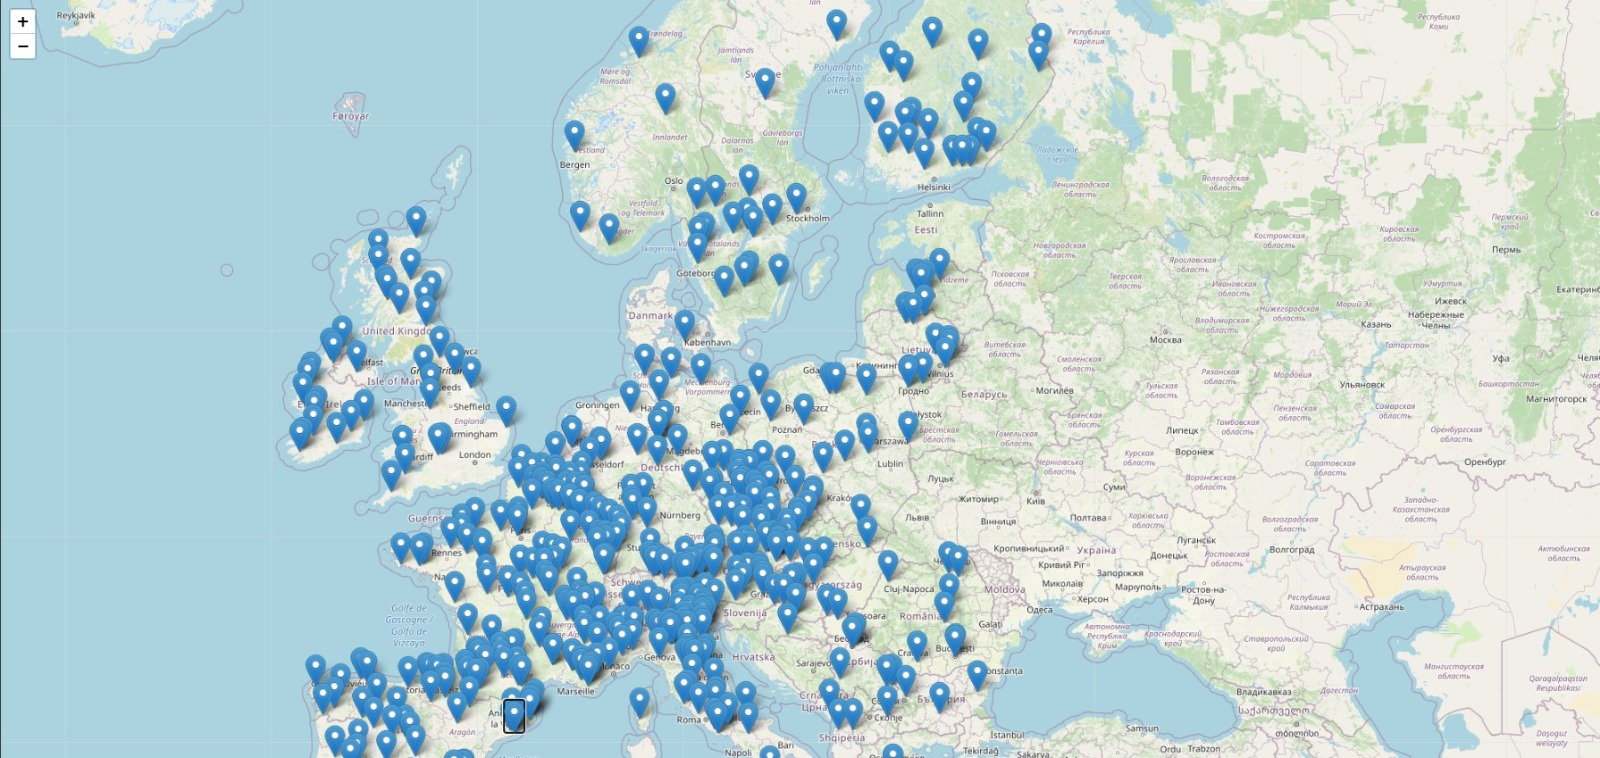
\includegraphics[width=11cm]{first500Row.jpg}
\end{figure}
\subsection{Predictive Models}
Our main problem was a regression problem because of the data we chose. "resulltMeanValue", which is our target feature, contains continuous values. However, we handled the problem both as a classification and regression problem.
\subsubsection{Classical Classification Algorithms}
For the classification problem, we first chose to use classical ML algorithms. The algorithms we have chosen for this are XGBoost, KNN, SVC, Random Forest, Ada Boost and Naive Bayes. We created different models and trained and predicted with the same data. We made our target attribute categorical by specifying a threshold value. The models gave the following results.
\begin{table}[h]
\centering
\begin{tabular}{|l|l|l|}
\hline
\textbf{Model} & \textbf{Accuracy} & \textbf{ROC/AUC Score} \\ \hline
XGBoost        & 0.9892            & 0.9889                 \\ \hline
KNN            & 0.9877            & 0.9171                 \\ \hline
SVC            & 0.9867            & 0.9346                 \\ \hline
Random Forest  & 0.9906            & 0.9357                 \\ \hline
AdaBoost       & 0.9884            & 0.9836                 \\ \hline
Naive Bayes    & 0.6575            & 0.8351                 \\ \hline
\end{tabular}
\end{table}
\subsubsection{Regression}
When we wanted to solve the problem with a regression algorithm, we chose the XGBoost regressor, which is the favorite algorithm of Kaggle competitions. With the XGBoost regressor, we got the following results according to certain metrics.
\begin{table}[h]
\centering
\begin{tabular}{|l|l|}
\hline
\textbf{Metric}            & \textbf{XGBoost Regressor Score} \\ \hline
MSE                        & 26658.278980488074               \\ \hline
RMSE                       & 163.273633222666443              \\ \hline
R\textasciicircum{}2 Score & 0.14316101172408313              \\ \hline
\end{tabular}
\end{table}
\subsubsection{Classification by Features}
In line with the decision we made as a result of our interview in this section, we run the model by adding the features one by one to see how effective the features are. But the features did not affect the accuracy much.
\begin{figure}[h]
    \centering
    \includegraphics[width=8cm]{classificatiionByFeatures.jpg}
\end{figure}
\section{Results}
In line with our studies, we found that it was difficult to collect data from the very beginning and work with them. We could not achieve the results we wanted in models resulting from our data selection. Even though we get high scores, we think it's overfit. In the following days, we will do tests with unseen data and we will make the models even better.
\section{Conclusion}
As a conclusion, it was a fun project for us. We used APIs that we did not use, did long-term research for data, and created a data set from scratch. This added a lot to us. We hope this project can go further.
\end{document}
